\documentclass[border=3pt]{standalone}
% Preâmbulo compartilhado pelos diagramas TikZ da aula 11 (Localização por Grade e Monte Carlo)
\usepackage[T1]{fontenc}
\usepackage[utf8]{inputenc}
\usepackage{lmodern}
\usepackage{amsmath}
\usepackage{xcolor}
\usepackage{tikz}
\usetikzlibrary{arrows.meta,angles,quotes,decorations.pathmorphing,calc,
                positioning,shapes.geometric,shapes.misc,backgrounds,fit,
                math}

% Paleta (mesma dos SVGs originais)
\definecolor{dblue}{HTML}{2A5B8C}
\definecolor{dorange}{HTML}{B3541E}
\definecolor{dgreen}{HTML}{4A7C59}
\definecolor{dred}{HTML}{9C4B4B}
\definecolor{dcream}{HTML}{F4F1EA}
\definecolor{dshade}{HTML}{DDD7C9}

% Função gaussiana (não normalizada por padrão de escala visual)
\pgfmathdeclarefunction{gauss}{3}{%
  \pgfmathparse{1/(#3*sqrt(2*pi))*exp(-((#1-#2)^2)/(2*#3^2))}%
}

% Estilos comuns (prefixo d... para não colidir com chaves internas do pgf)
\tikzset{
  >={Stealth[length=2mm]},
  dguide/.style={gray!55, dashed, line width=0.4pt},
  daxis/.style={gray!60, line width=0.7pt, ->},
  dbody/.style={fill=black!3, draw=black!80, line width=1pt},
  dacc/.style={draw=dblue, line width=1pt},
  dlbl/.style={black!55, font=\small},
  dsub/.style={black!45, font=\footnotesize},
  dstate/.style={circle, draw=black!80, fill=dcream, line width=1pt,
                 minimum size=17mm, font=\large, inner sep=1pt},
  dobs/.style={circle, draw=black!80, fill=dshade, line width=1pt,
               minimum size=14mm, font=\large, inner sep=1pt},
  dbox/.style={rounded corners=2pt, draw=black!80, fill=dcream, line width=1pt,
               align=center, inner sep=6pt},
  dop/.style={circle, draw=black!80, fill=white, line width=1pt,
              minimum size=6mm, inner sep=0pt, font=\small},
  dtrans/.style={->, dblue, line width=1pt},
  dmeas/.style={->, dorange, line width=1pt},
  dcurve/.style={line width=1pt, dblue},
  dcurveb/.style={line width=1.4pt, dorange},
}

\begin{document}
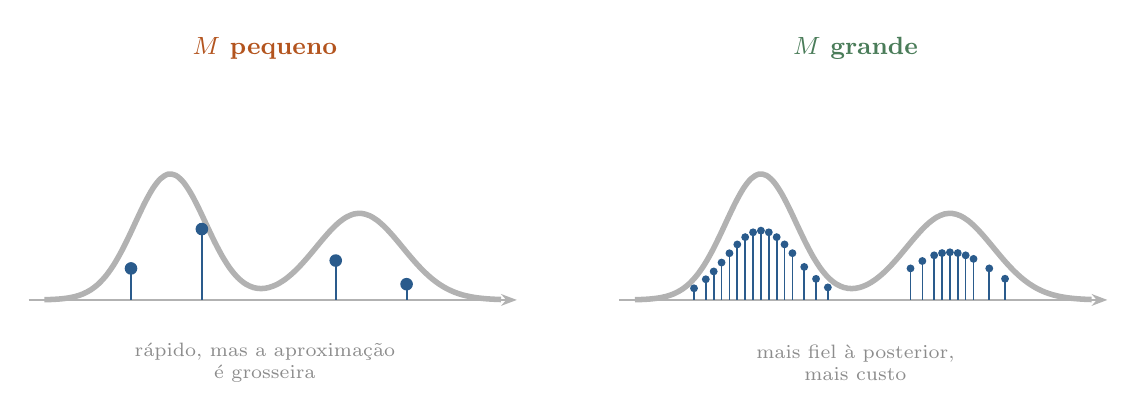
\begin{tikzpicture}[x=1cm,y=1cm]
  \newcommand{\alvo}{\draw[daxis] (0,0) -- (6.2,0); \draw[black!30, line width=2pt, domain=0.2:6, samples=60, smooth] plot (\x, {1.6*exp(-((\x-1.8)^2)/(2*0.45^2))+1.1*exp(-((\x-4.2)^2)/(2*0.55^2))});}
  \begin{scope}
    \alvo \node[font=\small\bfseries, dorange] at (3,3.2) {$M$ pequeno};
    \foreach \x/\h in {1.3/0.4,2.2/0.9,3.9/0.5,4.8/0.2} { \draw[dblue, line width=0.7pt] (\x,0) -- (\x,\h); \fill[dblue] (\x,\h) circle (0.08); }
    \node[dsub, font=\scriptsize, align=center] at (3,-0.8) {rápido, mas a aproximação\\ é grosseira};
  \end{scope}
  \begin{scope}[shift={(7.5,0)}]
    \alvo \node[font=\small\bfseries, dgreen] at (3,3.2) {$M$ grande};
    \foreach \x in {0.95,1.1,1.2,1.3,1.4,1.5,1.6,1.7,1.8,1.9,2.0,2.1,2.2,2.35,2.5,2.65,3.7,3.85,4.0,4.1,4.2,4.3,4.4,4.5,4.7,4.9} {
      \pgfmathsetmacro{\h}{0.55*(1.6*exp(-((\x-1.8)^2)/(2*0.45^2))+1.1*exp(-((\x-4.2)^2)/(2*0.55^2)))}
      \draw[dblue, line width=0.6pt] (\x,0) -- (\x,\h); \fill[dblue] (\x,\h) circle (0.05);
    }
    \node[dsub, font=\scriptsize, align=center] at (3,-0.8) {mais fiel à posterior,\\ mais custo};
  \end{scope}
\end{tikzpicture}
\end{document}
